\ifx\justbeingincluded\undefined
\input chappreamble.tex
\input foolthesis.tex
\fi

\chapter{Detecting Collisions}
\label{chapter:collisions}

%\section{Molecular Collision Theory}

Collisions are an exciting area of study for low temperature molecular systems. 
Quantization of intermolecular degrees of freedom leads to a host of interesting dynamics, which until relatively recently could only be discerned via their contribution to measured integrated cross sections including averaging over many initial states and many partial waves of the interaction potential.
However, with the ability to isolate single quantum states thanks to selective manipulation techniques, and with the reduction of collision energies afforded by deceleration, new state-resolved effects~\cite{Greenberg2018}, and new resolution on quantum mechanical interference type effects are now achievable~\cite{Zastrow2014,Klein2016}.
It is even possible to study effects directly pertaining to the orientation or stereodynamics of molecular interactions~\cite{Perreault2017}.
Simultaneously, studies of collisions in traps have evolved from total cross section measurements~\cite{Sawyer2008,Wiederkehr2012}, to lower temperature determinations directly relevant to inelastic-elastic ratios~\cite{Marx2015,Wu2017,Segev2019}.

This last result~\cite{Segev2019} from the Narevicius group is particularly exciting, as it compares quite directly with our own work, including cryogenic skimming techniques, decelerator optimization, and cryogenic trapping optimization, and is worth further discussion here.
Realizing a similar observation would be an exciting outcome of the research in this thesis, though at the time of this writing it remains unclear whether the optimizations we have pursued will achieve densities comparable to~\cite{Segev2019}. 
In their Zeeman deceleration of oxygen, benefit is taken from oxygen's much more direct sourcing, and from the better integration of skimmer cooling with Zeeman deceleration thanks to the possibility of affixing a long cryogenic Sapphire tube within the bore of the decelerator\footnote{In private communication with Yair Segev, we discussed the application of skimmer cooling to deceleration, and the use of such tubes in the Narevicius group.}~.
In contrast, for OH our discharging yield from water may be only $1-10$\%, and skimmer cooling has only led to two-fold gains with the hexapole~\ref{chapter:focusing}.

Another alternative strategy for phase space compression of molecules applicable to a wide array of species is found in the combination of centrifugal deceleration and optoelectric cooling~\cite{Prehn2016}.
The deceleration technique has also directly enabled collisional studies on its own~\cite{Wu2017}, of $\text{CH}_3\text{F}$ and ND$_3$.
The optoelectric sisyphus technique requires low spatial density flat-bottomed trap geometries, but the velocity space compression is quite impressive, $420^\circ~\!\mu$K is reached.
Laser-based techniques are also beginning to enable similar molecular collisional studies, notably the recently observed sympathetic cooling of NaLi molecules by sodium~\cite{Park2019}, the first successful sympathetic cooling of a molecule by an atom.
Work on laser-cooled molecules has also recently progressed to the collisional stage, with the Doyle group reporting on collisions between pairs of CaF molecules loaded into optical tweezers~\cite{Anderegg2019}.

A key challenge that has emerged during the course of my thesis work has been the verification of collisional behavior of all kinds.
For this purpose, several very general techniques exist, which are now described in detail.

\section{Controlled Density Reductions}

Collisional effects always influence a population in proportion to the likelihood of such collisions, which in turn scale with the square of the number density of the population.
It therefore follows that as one were to scale an experimental control parameter tuning the number density of the population, collisional effects would grow quadratically in that parameter, while single-particle effects would grow linearly.
The challenge lies in whether it is really possible to achieve a tuning of this parameter which does not inadvertently lead to an unwanted change of a different nature.
Several different strategies have been pursued in this regard.
The molecule source is perhaps the most logically natural place to begin, but in practice all ways of tuning the initial molecule density risk disturbing the experiment in unwanted ways.
For example, tuning the current of the discharge filament can easily reduce the measured number of molecules, and is simple to control and manipulate, but its most likely method of action is to make the discharging process more sporadic, in which case the measured reduction may actually be dominated by cases where no molecules are generated at all.
In this scenario, densities remain as always, but some fraction of the time the discharge fails to ignite and no molecules are produced at all.
This situation may masquerade as a density tuning, but in fact does not at all investigate the physics of interest.

Other source parameters include the stagnation pressure in the pulsed valve; parameters influencing the flux of the opening event such as coil current, coil voltage, pulse duration; or valve temperature.
In all of these cases, there is the risk that changes in the number of molecules generated can change the efficiency of the supersonic expansion process, thereby changing the molecule distribution function across the population, and not only its number density.
If we were verifiably operating in a regime where the valve dramatically overfills the decelerator's phase space acceptance, these effects could more plausibly be neglected, but this assertion is not justified, especially when seeking small effects and when using the relatively narrow initial distribution of the Even-Lavie valve.
To be more concrete, let us parametrize the most likely way that phase space distributions resulting from different source parameter changes may vary from one another.
Assuming that in all cases we at least maximize the signal loaded into the decelerator as far as it depends on timing parameters, we can approximate the phase space distribution downstream in the decelerator where many rotations have cleaned out variations in the angular coordinate as follows:
\begin{equation}
\delta(r) = e^{-\frac{r^2}{2\sigma_r^2}},\label{eqbaddist}
\end{equation}
where $r$ is defined for a planar space-velocity slice of phase space as:
\begin{equation}
r^2 = (z-z_0)^2 + (v_z-v_0)^2/\omega^2,
\end{equation}
$z_0$ and $v_0$ are the center coordinates of the phase space distribution, and $\sigma_r$ parametrizes the width of the distribution.

Variations in this $\sigma_r$ can eventually contribute to subtle influences in the observed lifetime of the gas, since $\sigma_r$ in turn influences the extent to which the outer reaches of the trap are populated after loading.
Source variations which change the initial temperature of the supersonic expansion are likely to increase the value of $\sigma_r$, leading to greater population in the wings, and faster decay rates early on during loading, a classic indicator of collisional effects, which also lead to faster decays early on which later turn off as the population reduces.
The distribution proposed in Eq.~\ref{eqbaddist} is in fact a more benign representation of what is possible.
Loading a narrow distribution off of center can easily lead the radially averaged phase space distribution to actually peak away from center for example.

\figdave{uwprobe}{Microwave Free Space Coupling Probe}{
A microwave free space coupling probe used for addressing OH molecules even in the midst of the Stark decelerator.
The brass structure is in good mechanical and electrical contact with the center pin of a coaxial vacuum feedthrough mounted in a 2.75" conflat vacuum connector.
This is achieved with the 0-80 setscrew just visible towards the base of the brass structure.
The thin region of the Brass structure has a 1/4" diameter, and the thick region is closer to 3/4" diameter.
}{12cm}

Another possibility for achieving density variations without changing the distribution $\delta(r)$ of molecules delivered eventually to the trap is to perturb some aspect of the deceleration process, but leave the source untouched.
Any phase space manipulation based technique, such as operating in different deceleration modes or introducing gaps in the coverage of the traveling potential, would have the same possibility of disturbing the distribution ultimately loaded into the trap as just described for the case of source variations.
However, in the decelerator, the population is already state selected, opening up the different possibility of directly reducing the density by spectroscopic means.
Were a second LIF laser available and a region of good optical access before the trapping region, this would serve as a reliable means to achieve a $50\%$ density reduction for example, although at the expense of writing intensity noise and other shot-to-shot variation issues of the pulsed dye laser onto the number density of the ensemble.
Microwave transfer is a more compelling possibility, especially since it affords the possibility of directly transferring molecules to an un-trapped state.
Applying them during deceleration presents a bit of a challenge however, especially given the usual engineering constraints imposed by the high voltage system.
In the past, we've addressed this using the biased tee strategy described further in~\cite{Stuhl2012uwave}, but hoping for a simpler workaround, we attempted a microwave near-field probe coupler as shown in Fig.~\ref{uwprobe}.

\figdave{uwaveproof}{Successful Coupling of Free-Space Microwave Cavity Modes}{Microwaves are successfully coupled into our vacuum chamber using the probe shown in Fig.~\ref{uwprobe}, as evidenced by the response of hydroxyl radicals to increasing powers shown here.
These molecules were slowed to $43$~m/s and then allowed to fly through the detection region with no trap loading.
These data were collected on June 14th, 2016.
Microwave powers are as measured at the vacuum feedthrough.
At a later point, we were able to apply even higher RF powers by instead applying them in a pulsed manner so as to remain within the capabilities of our microwave equipment.
Fitted FWHM values in $\mu$s are reported in the legend and found not to vary with power.}{\linewidth}

In the microwave engineering literature~\cite[Sec.~4.7]{Pozar2009}, a probe is a near-field device used either for driving a waveguide or measuring its local field behavior. 
The chamber in which our decelerator sits has a $20$~cm diameter, comparable to the microwave frequencies relevant for driving \f3 to \e3 transitions, where in zero field $1.7$~GHZ corresponds to $18$~cm wavelengths, so it is reasonable to expect that a simple current probe might successfully drive microwave modes of the vacuum chamber.
This indeed turns out to be the case, and we successfully used this probe, not only for microwave removal of population during deceleration, as shown in Fig.~\ref{uwaveproof}, but also to perform the same in-trap spectroscopy described in the previous chapter.

\section{Fitting Trap Decay Curves}

Another competing technique for observing the influence of collisions relates to the functional form of the decay that is exhibited from a trapping geometry as a function of time.
If we make the na\"{i}ve assumption that collisions lead to loss uniformly over a population regardless of other parameters, this can be described by the following differential equation:
\begin{equation}
\frac{dN}{dt} = - \beta N^2  -\alpha N,
\end{equation}
where the magnitude of the two-body process is parametrized by $\beta$, and single-particle effects such as collisions with background gas molecules are included in the model and parametrized by $\alpha$.
This can in turn be solved by the factorization method for rational polynomial functions:
\begin{eqnarray}
\int\frac{dN}{N(\alpha+\beta N)} &=&- t + C,\\
\int\frac{1}{\alpha}\left(\frac{1}{N} - \frac{\beta}{\alpha +\beta N}  \right)dN &=& -t+C\\
\log{N} - \log{\left(\alpha + \beta N\right)} &=& -\alpha t + C'\\
\frac{N}{\alpha + \beta N} &=& C''e^{-\alpha t}\\
\frac{1}{\alpha/N + \beta} &=& C''e^{-\alpha t}\\
\alpha/N + \beta &=& C'''e^{\alpha t}\\
N(t) &=& \frac{\alpha}{C'''e^{\alpha t}-\beta}
\end{eqnarray}
Now by requiring that $N(0)=N_0$, we have:
\begin{eqnarray}
N_0 = \frac{\alpha}{C'''-\beta}\\
C''' = \frac{\alpha}{N_0}+\beta.
\end{eqnarray}
Substituting and moving around:
\begin{eqnarray}
N(t) &=& \frac{\alpha}{(\frac{\alpha}{N_0}+\beta)e^{\alpha t}-\beta}\\
&=& \frac{N_0 e^{-\alpha t}}{1 +\beta N_0(1-e^{-\alpha t})/\alpha}\label{eq12body}
\end{eqnarray}
This equation is rather ugly, but it can be seen to reduce to the more well known formulas describing the decay of a population subject to either single or double particle effects but not both.
To see this, we simply take the corresponding $\alpha$ or $\beta$ parameters in Eq.~\ref{eq12body} to zero:
\begin{eqnarray}
\lim_{\beta\rightarrow 0} \left(\frac{N_0 e^{-\alpha t}}{1 +\beta N_0(1-e^{-\alpha t})/\alpha}\right) &=& N_0 e^{-\alpha t}\\
\lim_{\alpha\rightarrow 0} \left(\frac{N_0 e^{-\alpha t}}{1 +\beta N_0(1-e^{-\alpha t})/\alpha}\right) = \frac{N_0}{1+\beta N_0 \left( te^{-\alpha t}|_{\alpha=0} \right)} &=& \frac{N_0}{1+\beta N_0 t} \label{2bodyeq}
\end{eqnarray}
where the penultimate step for the two-body formula is achieved via L'H\^{o}pital's rule.

With these functional forms in hand, it is now possible to use the fitting of measured trap decays as an observable giving indication of the presence of collisional effects.
Historically, this procedure was used in our experiment in both the Ring and Tricycle traps, but never in the Pin trap due to thanks to the development of our capability of performing controlled density reductions.
When using decay fits, it is essential that these observations are made in the absence of any time varying single-particle loss processes, such as the potentially slow escape dynamics of some classes of molecules from the trap geometry.
In the Ring trap for example, we have experimental indications that molecules do not explore the toroidal region of the trap, although they have access to it.
This confirms that the ensemble loaded in this trap is in a potentially dangerous regime for the application of loss functional forms, since there should certainly be a timescale for molecules to explore the toroid which has not been easily satisfied in the first few milliseconds after trap loading.

I can take this a step further by approximating a trap with slow escape dynamics for some populations as one characterized by two different single-particle decay times:
\begin{equation}
N(t)=A_1e^{-\alpha_1 t} + A_2e^{-\alpha_2 t}
\end{equation}
Now consider a trap where half the population decays with a background pressure limited lifetime of $500$~ms and the other half escapes the trap on a timescale that is slow relative to a $300~\mu$s oscillation time but faster than the background limit, say $50$~ms.
These numbers are somewhat representative of historical values in our traps.
In the absence of any collisional effects, fitting this bi-exponential decay with Eq.~\ref{eq12body} is optimal with a zero-valued $\alpha$, and with $\beta=9.9\pm0.1$/s/mol. 
Not only does the hypothesis of decay according to Eq.~\ref{eq12body} give a strong slant in favor of two-body effects, it does so with high fidelity, fitting the data with an $R^2=0.99$, see Fig.~\ref{biexp2body}.
I should mention that in this fitting I fix the initial population to one, which reduces the ability of Eq.~\ref{eq12body} to fit any arbitrary shape.

\figdave{biexp2body}{Decay Fitting for Collision Rate Extraction}{A biexponential decay curve is well fit by a two body, demonstrating the importance of either removing single-particle effects or ensuring that they occur on only a single timescale.}{\linewidth}

Of course one contributing factor to the success of the two-body fit in matching the biexponential decay curve is the timescale probed in the experiment.
One more effective way for distinguishing true two-body effects could be to use a long-time measurement to fix the one-body decay rate, since at long enough times the two-body effects reduce in relevance while the one-body rates remain fixed.
In practice, this approach can lead to more trouble, since at about $3$~s~\cite{Hoekstra2007}, an additional one-body process kicks in, but as long as one-body effects are well-known, pushing to long timescales can improve the reliability of the decay-fitting method for detecting collisions.

\subsection{Electric Field Induced Losses}\label{sec:efil}

One area where the fitting of decay curves played a very large roll was in the study of what was thought to be electric field induced inelastic loss.
In the experiment~\cite{Stuhl2013}, it was found that application of electric field led to loss from the trap. 
It was further found that initiating the loss after different hold times in the trap was a way of varying the initial density so as to probe the two-body process in different parameter regimes.
Some example fits from~\cite{Stuhl2013} are shown in Fig.~\ref{efielddecay}a.
At the time, it was known that a single particle loss due to electric field existed, discussed in the appendix of~\cite{Stuhl2013}.
Its magnitude was approximated, and fixed in Eq.~\ref{eq12body} when fitting decay curves.
It was argued that this strategy of fitting Eq.~\ref{eq12body} while varying initial population would lend robustness to the procedure despite the known difficulties of relying on Eq.~\ref{eq12body}~\citep[Page.~1800, bottom right]{Stuhl2013}.

\begin{figure}[t!]
\centering
\vspace{0.5mm}
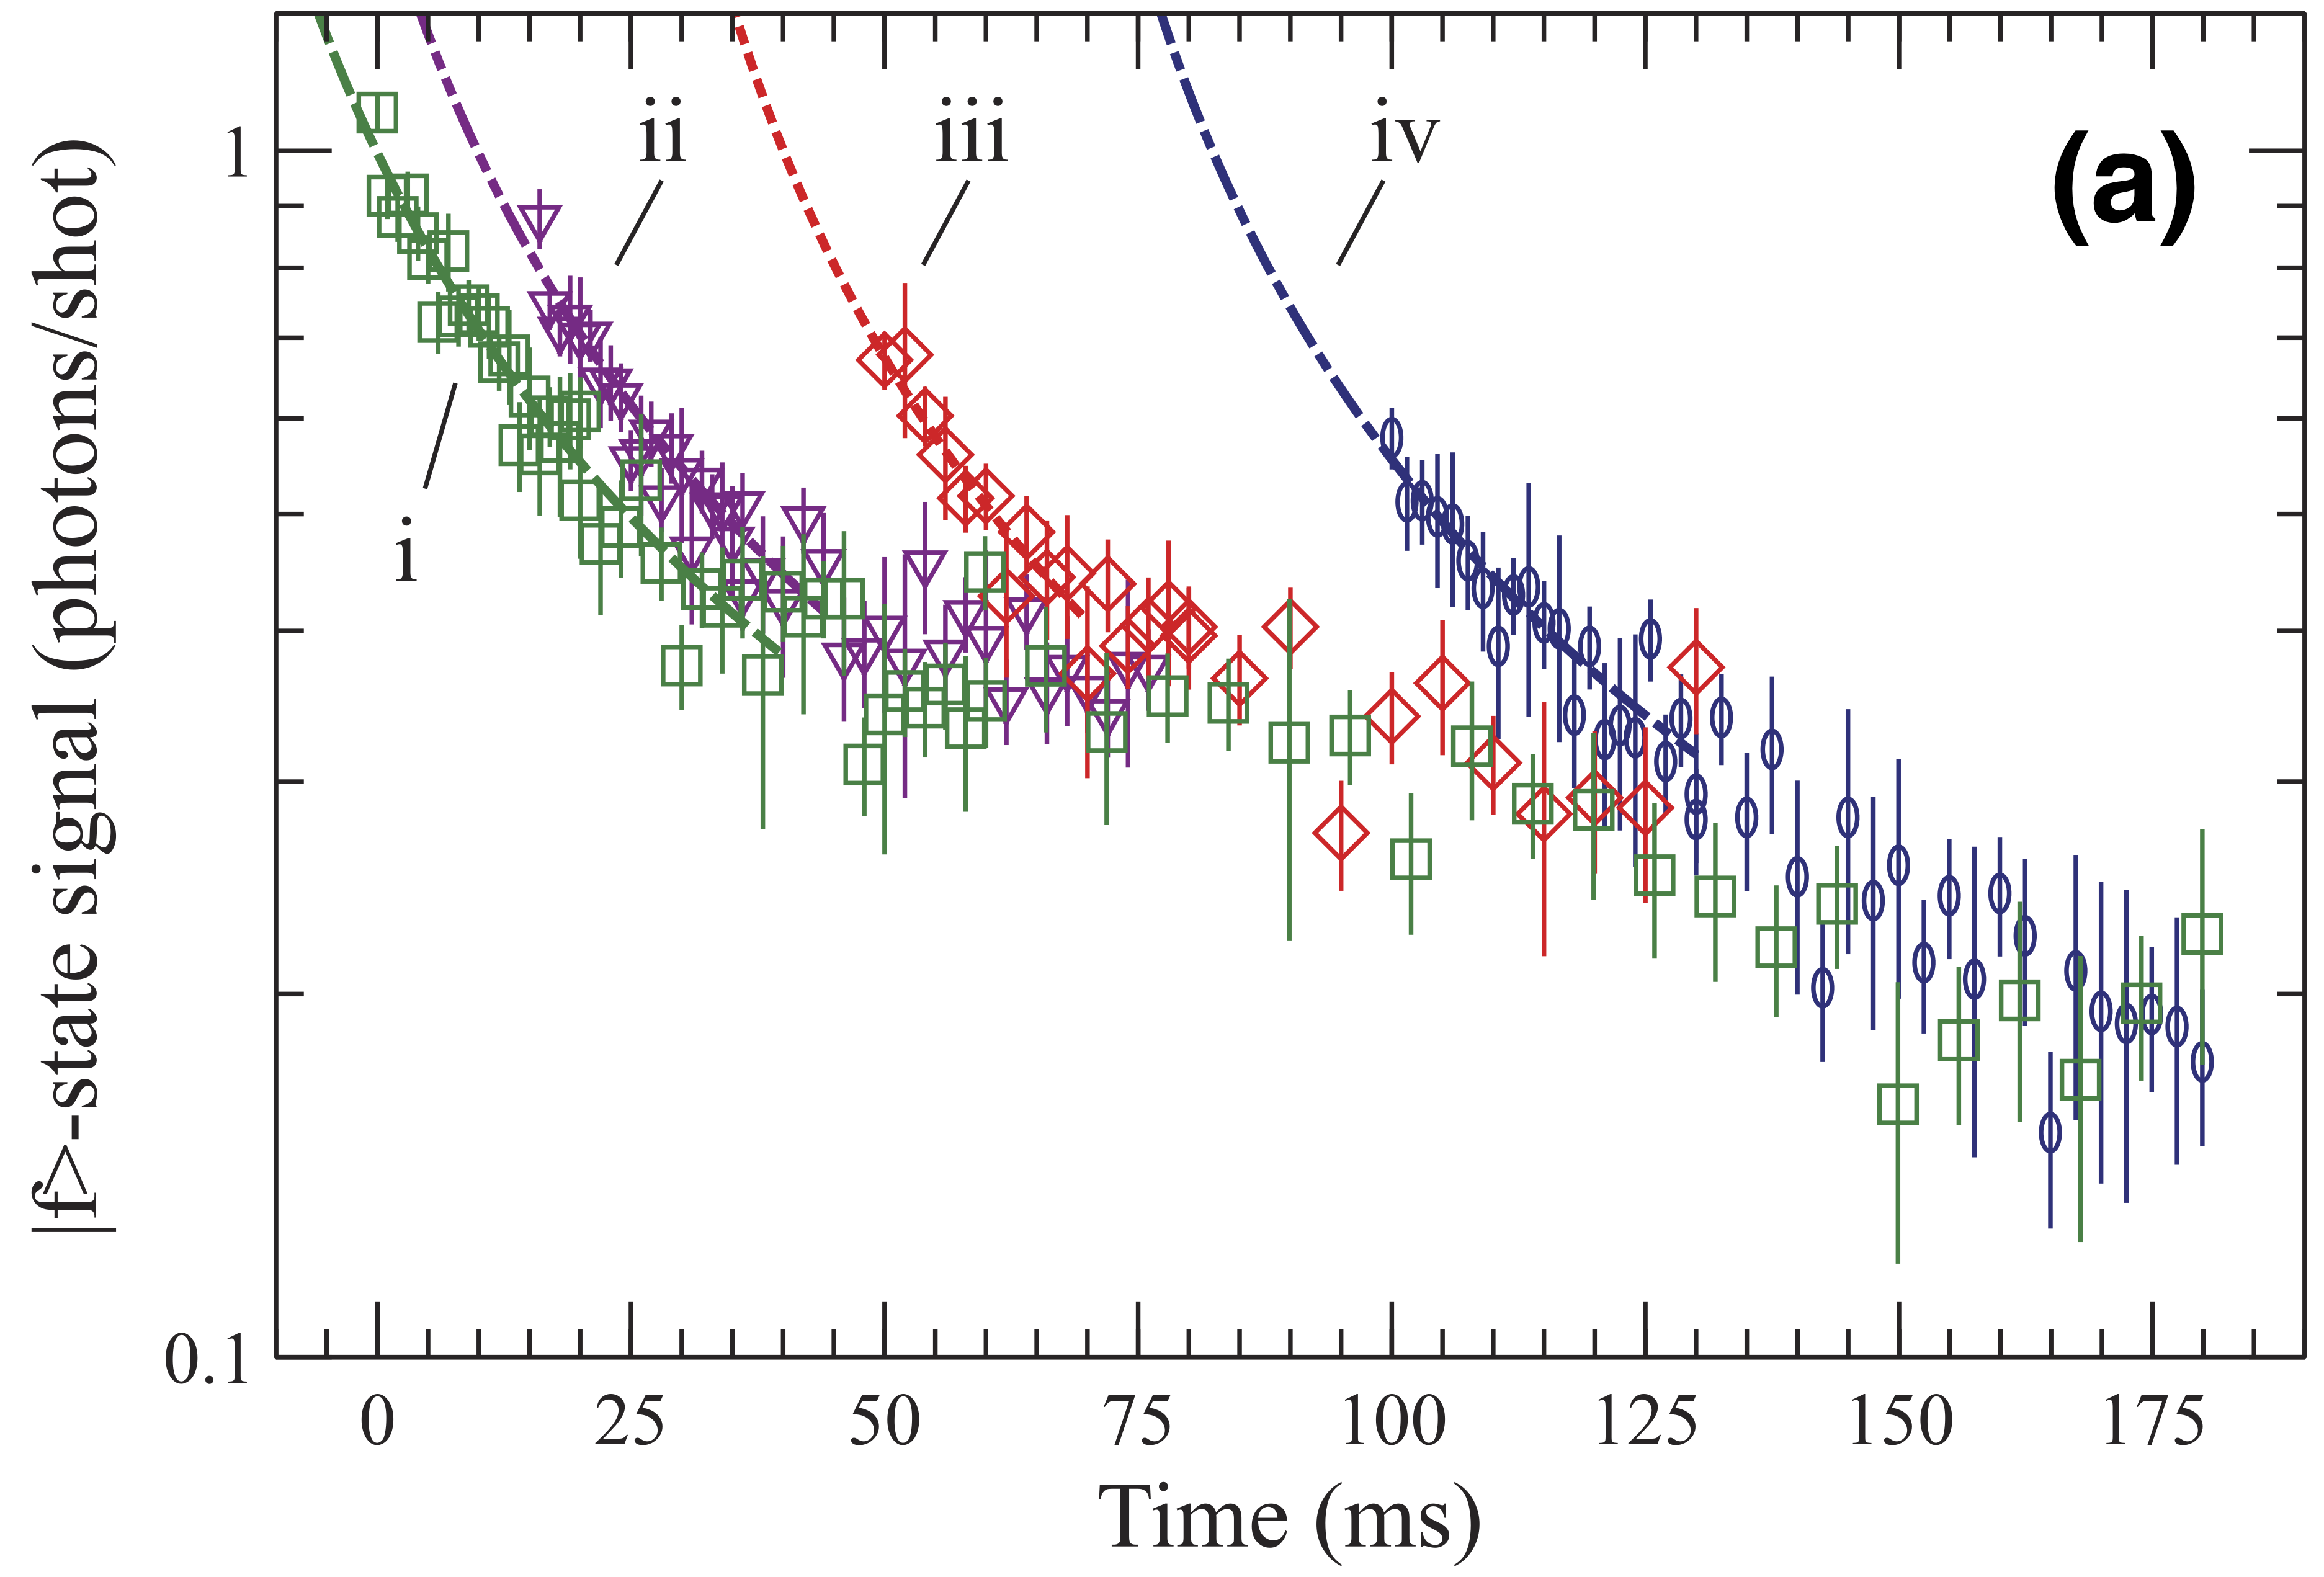
\includegraphics[width=10cm]{stuhlinelastic}
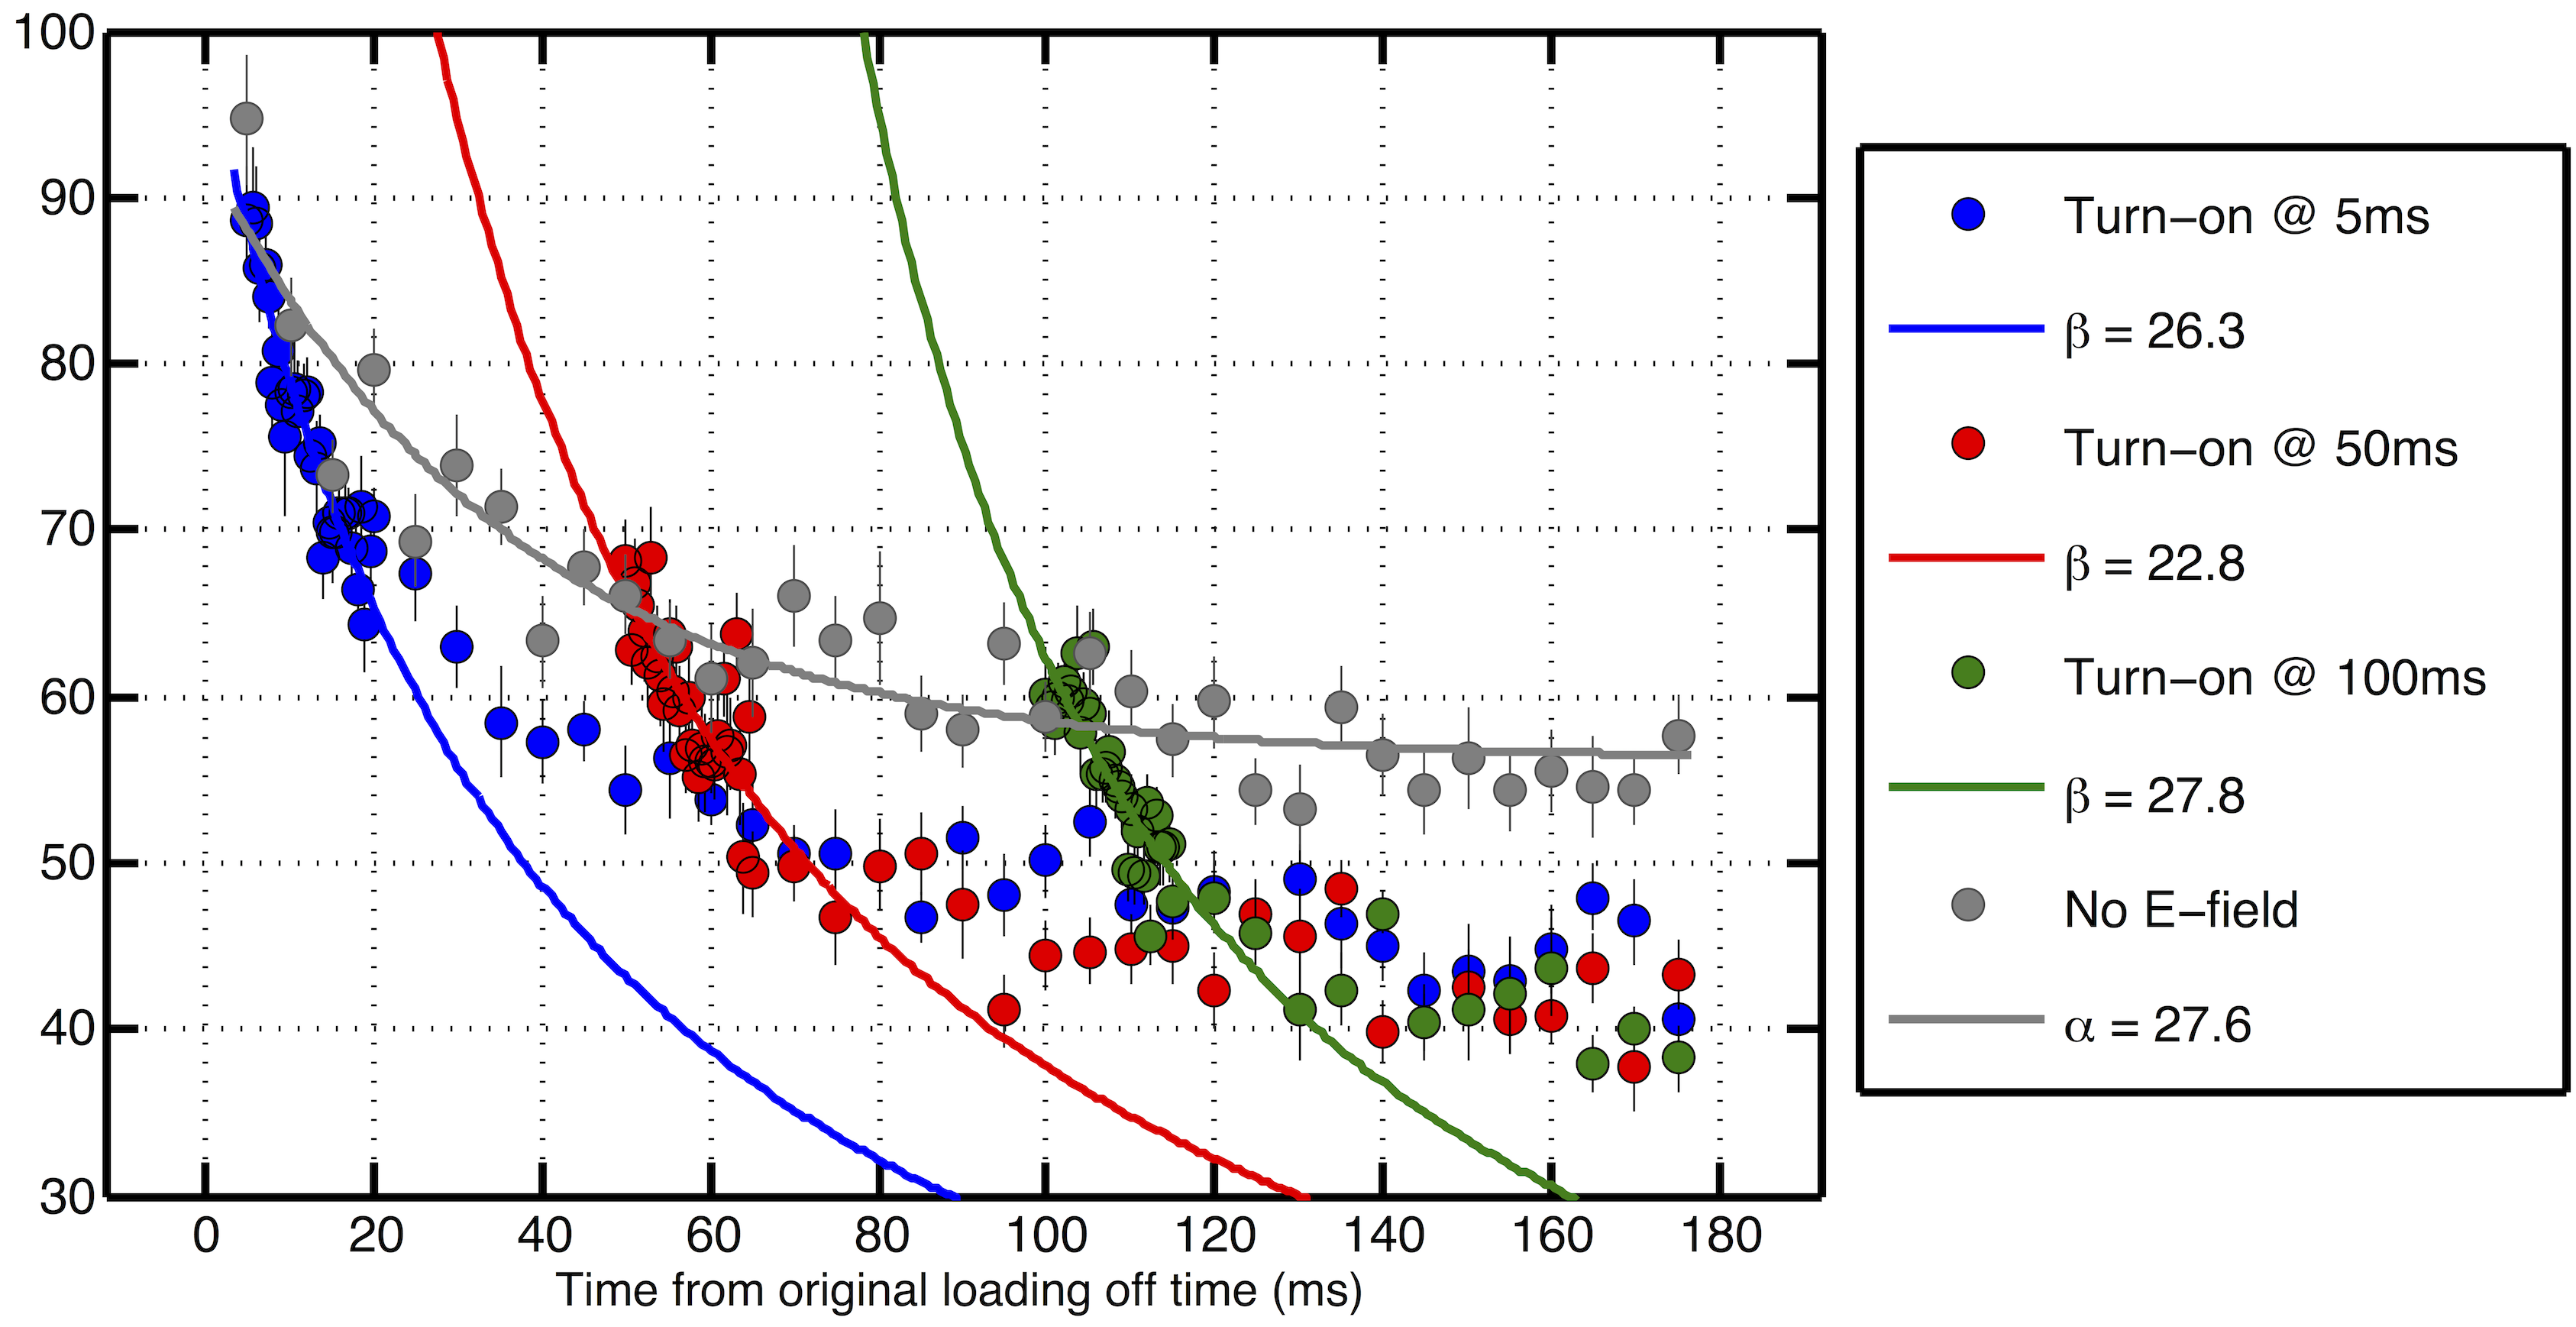
\includegraphics[width=14cm]{reensinelastic}
\caption[Electric Field Induced Decays]{
Electric field induced decays with different turn-on times of the electric field are shown.
(a) Fits to decays initiated after application of a $3$~kV/cm electric field after different wait times yield two body parameters $\beta$ of (i) $40.4\pm3.0$, (ii) $41.2\pm4.2$, (iii) $48.4\pm8.1$, and (iv) $45.4\pm5.5$ (photons/shot)$^{-1}$s$^{-1}$. 
Intrigued by the data shown in panel (a) from~\cite{Stuhl2013}, we took data with an emphasis on simultaneous collection for reduced systematics at longer timescales for all datasets, resulting in panel (b), collected in March of 2014 in the Tricycle trap with a similar electric field magnitude.
\label{efielddecay}}
\end{figure}

During our reinvestigation, we pushed the decay measurements out to long times, and found the results shown in Fig.~\ref{efielddecay}b.
These results are a big challenge to the hypothesis of a fixed single particle loss timescale, and strongly suggest a time-dependence of the single particle loss, since there is no reason that either a one-body or two-body effect, initiated after various wait times, should lead to nearly overlapped traces in the long term.
Note how near $180$~ms in Fig.~\ref{efielddecay}b, the $50$, $100$, and $150$~ms traces all approach the same level.
Intrigued by this observation of what seemed like a fixed magnitude trap-loss induced by the turn-on of the electric field, we also experimented with the application of multiple pulses of electric field, and obtained the results shown in Fig.~\ref{efieldmulti}.
This presents an additional challenge to the hypothesis of simple electric field dependent loss parameters, which ought to respond only to the time integrated electric field application, and not whether it is pulsed or continuous.
In contrast, in Fig.~\ref{efieldmulti} we find that applying the electric field for the entirety of the time sequence (red) causes far less loss than applying it for half of the time, but in a switched manner (yellow).
This is strongly suggestive of a dynamical effect, i.e. an effect which concerns the short term dynamics of molecule trajectories in their trapping potential, and not a collisional effect which ought to respond generally speaking to thermodynamically and temporally averaged quantities.

\figdave{efieldmulti}{Multiple Electric Field Applications}{
Trap decay curves under various conditions related to the timing of application of electric field.
The conditions are (blue) no electric field applied, (red) constant electric field applied, (yellow) $5$~ms pulses of electric field every $10$~ms.
Lines are five point running averages.
Data collected in March of 2014.
}{\linewidth}

Specifically, one obvious dynamical effect would be the behavior of the population in the presence of a spin-flip loss region, discussed at length in Sec.~\ref{sec:mech}.
Molecules whose orbits regularly intersect the loss region are lost, but molecules may exist whose orbits never intersect the loss region.
Indeed, such a class of molecules is mathematically guaranteed, thanks to the cylindrical symmetry of the ring and tricycle trap. 
This symmetry enforces the conservation of angular momentum about the axis of cylindrical symmetry under the evolution of the classical Hamiltonian governing molecular trap orbits.
Since the loss region occurs close to this axis, molecules with enough azimuthal angular momentum never intersect the loss region under classical Hamiltonian trajectory evolution.
With some collisional thermalization however, trajectories which intersect the loss region should gradually be repopulated, but at a rate that is slow relative to the initial escape dynamics.
We can conclude that if thermalization is slow, electric field enhanced spin-flip loss can cause a decay rate that decreases over time.
If thermalization is slow even compared to the total experiment runtime, spin-flip loss should lead to the removal of a fixed subset of the population over a certain dynamical timescale, regardless of any hold-time, exactly as observed in the long-term behavior in Fig.~\ref{efielddecay}b.

\section{Comparison to Simulation}

Comparison to simulations is a potentially favorable strategy for detecting the roll of collisions in an experiment.
Fast mean-field based approaches to simulating collisional gases exist, with that due to Bird~\cite{Bird1976} quite common in the literature.
In the course of this thesis, significant simulation endeavors were pursued, often exactly with this goal of elucidating the relative contribution of single and double particle effects.
Simulation is particularly promising in light of the role of dynamical effects described in the previous section, since any analytical forms are hopeless to shed light on dynamics, while the simulation should serve well with a suitably meshed trapping potential.

Firstly, a note of caution is in order.
Similar to the fitting of decay curves, comparison to simulations can be plagued by the same sorts of fundamental flaws as are the comparison to decay fits discussed in the last section.
The simulation should certainly perform better than analytic decay fits in that it does not need to make any homogeneous population or related assumptions, but at the expense of abandoning these homogeneity assumptions the simulation becomes dependent on many additional tuning parameters.
Extracted collisional contributions can strongly depend on these tuning parameters.
As a thought experiment, suppose that an experimental parameter like the trap strength, which may easily deviate between simulation and experiment due to manufacturing defects or variability in the permanent magnets for example, is indeed different between the simulation and the experiment. 
Suppose further that the simulation overestimates the trap depth by $10$\%.
This parameter is important for the short-time dynamics of molecules from the trap, and an overestimate would result in a reduced roll of these dynamics, leading the simulation to underestimate the initial decay rate due to dynamics.
Consequentially, it is likely that the best match between simulation and experiment would occur for a simulation with a larger number of collisions than the experiment, since these extra collisions would boost the initial decay rats to compensate for the trap depth overestimate.

These issues could be behind the incredibly large collision rates predicted in the simulation decay fitting shown in Fig.~\ref{decayfitex} for example.
These are not unperturbed decays, but occur during the application of various forced microwave evaporation sequences.
It is seen that large collision rates are rather successful at fitting the shapes observed in the trapping geometry.
A key parameter governing the comparison of simulation to experiment is the removal efficiency of the microwave knife, which could have dependencies on polarization and position in the trap that are not treated, dependence on molecule velocity, etc.
If this parameter is too small, the simulation will predict greater numbers of molecules remaining, and the collision rate will be reduced to match this, since the collision rate also influences molecule number remaining by influencing how successful the evaporation is.
I believe the match of microwave knife between simulation and experiment is responsible for the simulation landing at the large collision rate match of $130$~s$^{-1}$mol$^{-1}$ in Fig.~\ref{decayfitex}.

\figdave{decayfitex}{Extracting Collision Rates from Decay Fits}{
The fitting of the decays of molecules from the trap with direct Monte-Carlo simulations including collision rates are shown. 
Large collision rates of $130$/s are found to fit best, primarily due to the initially fast decay exhibited by the population.
These data were collected on June 26th, 2013.
The legend describes some details of the microwave knife, 
}{\linewidth}

In addition to parameter tuning, there is also the question of whether the simulation correctly includes all relevant effects, since simplifying assumptions are often essential for reasonable runtimes and development times.
Specifically, the influence of other substates of OH other than the doubly stretched one are pervasive and pernicious.
As discussed in Sec.~\ref{loadingtransitions}, molecules in the \fm3 state end up in either \f1 or \e3, and the dynamics of these molecules should also influence the dynamical escape processes involved during early trap decay.

\subsection{Simulating Electric Field Induced Loss}\label{sefil}

One key success achieved during my thesis work was the use of simulations to demonstrate the dynamical effects suggested by the experiments discussed above in Sec.~\ref{sec:efil}.
By carefully including the electric field enhanced spin flip loss in simulations but with no appreciable collision rate, and then applying the same fitting paradigm used in~\cite{Stuhl2013} to the decay traces obtained by simulation, a very close match is obtained to the experimental data, see Fig.~\ref{betaout}.
Each point corresponds to the fitting of a suite of decays occurring after different hold times at a specific electric field.
\figdave{betaout}{Successful Simulation of Electric Field Induced Loss}{
Two body fits from~\cite{Stuhl2013} to experimental data like that in Fig.~\ref{efielddecay} but at various electric fields. 
The blue data points and shaded region are repeated from Fig.~3 of~\cite{Stuhl2013}, where the shading indicates the variation that would be brought about by two-fold changes in the assumed one-body loss $\alpha$ from spin-flip losses.
The very close agreement highlights the ability of dynamical effects to masquerade as two-body decay curves.
}{10cm}
We can also examine the match of individual experiments, instead of only looking at the full collection.
An example of the simulated trajectories arising from a specific electric field is also shown in fig.~\ref{eilout}.
It is seen that the simulation overestimates the initial decay rate, but agrees fairly well with the total eventual loss.

\figdave{eilout}{Simulating Escape Dynamics After E-field}{
Experimental data on electric field-induced loss with an attempted overlap to spin-flip loss simulations. 
The case of no electric field (black, solid, circles) is compared to electric fields of $3\text{ kV/cm}$ turned on after a wait time indicated in the legend.
}{10cm}

At first it is perhaps tempting to attribute this discrepancy to the possible continued role of collisions.
However, there is no reason that collisions should influence this short time discrepancy, which is much more likely a higher order dynamical effect, especially since the dynamical effects were just seen to so nicely explain the observation of fixed total electric field induced loss.
And indeed, just such a higher order dynamical effect is available through the more careful inclusion of other substates of the OH ground state.
Electric field induced spin-flip loss does not directly remove molecules from the trap, but instead transfers them to lower lying states, some of which remain fairly well trapped.
This can be seen by viewing the energy of substates as a function of position in the trap, animated in Fig.~\ref{manysubstates}.
\begin{figure}[t!]
\centering
\vspace{0.5mm}
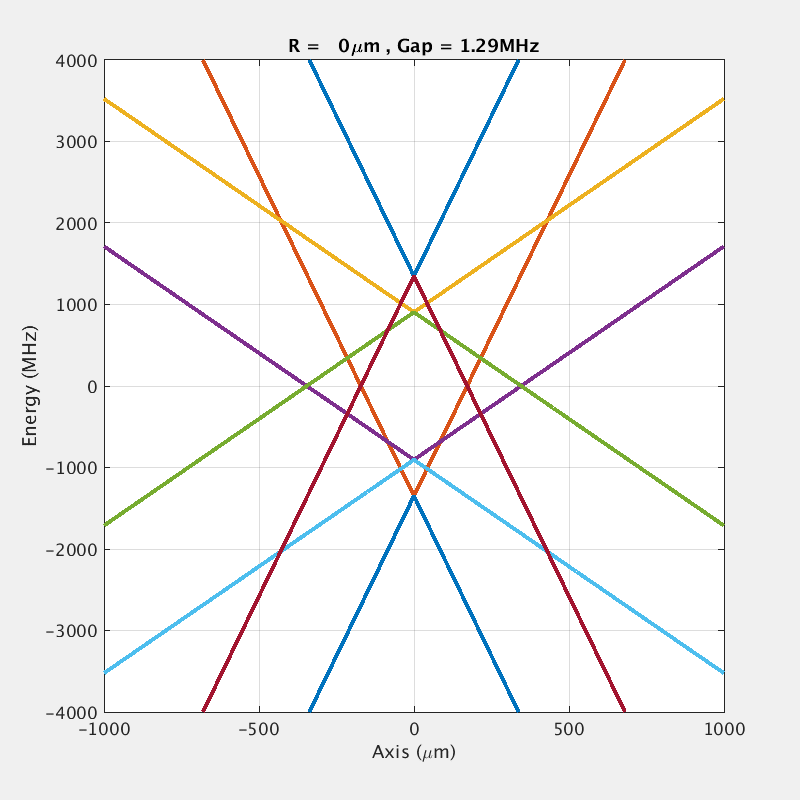
\includegraphics[width=8cm]{ohz0}
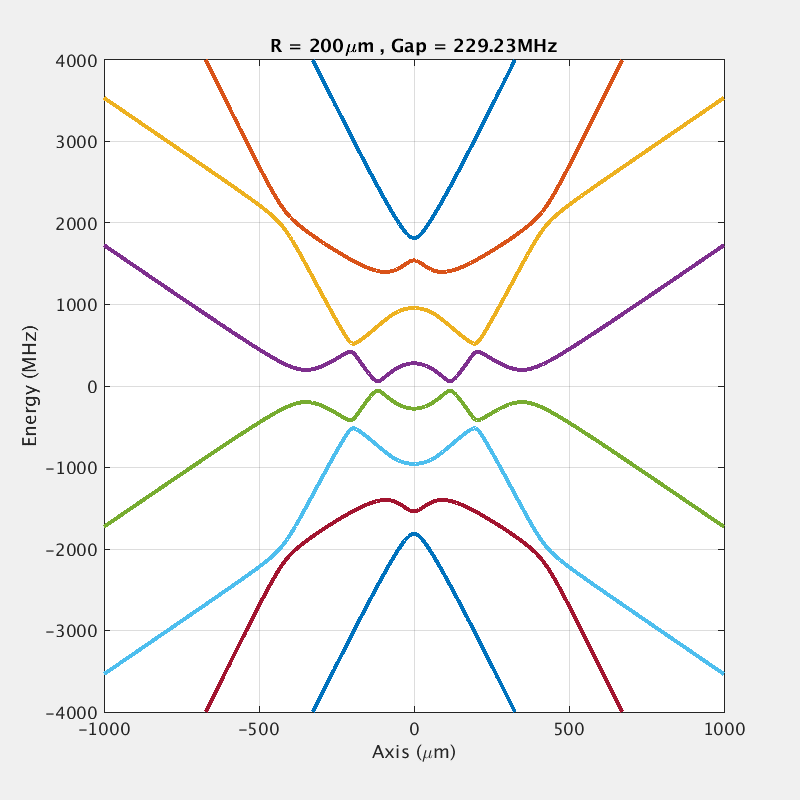
\includegraphics[width=8cm]{ohz2}\\
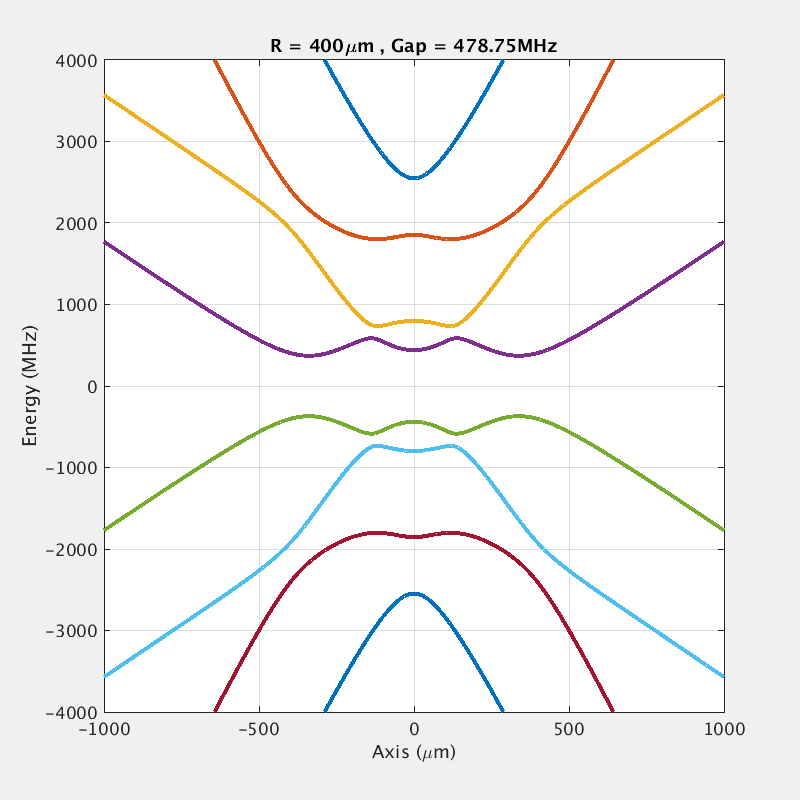
\includegraphics[width=8cm]{ohz4}
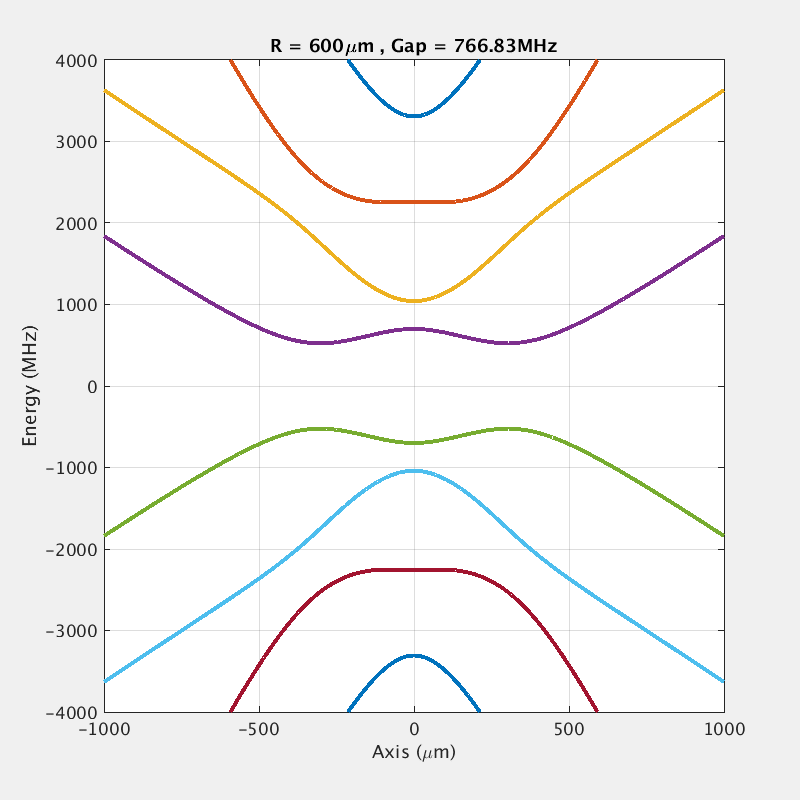
\includegraphics[width=8cm]{ohz6}
\caption[Partially Trapped Substates in Electric and Magnetic Fields]{
Eight ground states of OH as a function of position in a magnetic quadrupole trap with $3$~kV/cm applied.
In the top left, the energies of these eigenstates are plotted as a function of their position along the cylindrical axis through the quadrupole trap.
The doubly stretched state appears as a dark blue V near the center, and the other states may be identified based on their Zeeman effect at larger distances.
The red state is \e3, and has the same slope as the dark blue, yellow is \f1, purple \e1, etc.
In the other panels, position is plotted not along the axis, but parallel to it and offset by the distance labeled in the title of the panel, increasing in steps of $200~\mu$s.
The avoided crossings open up even for very small deviations from the axis, demonstrating that except for a few small openings, really the top four substates are predominantly trapped.
\label{manysubstates}}
\end{figure}
Along the axis, all states are connected, but as the radial coordinate increases, mostly trapped states separate away from the others.
Simulating this has several associated challenges.
Firstly, the dynamics associated with hopping between substates must be carefully treated.
This is made especially challenging by the fact that the location of hopping points between the second trapped substate and lower states varies with the magnitude of applied electric field, unlike the hopping point between the primary trapped state and the second, which is always located at the trap center.
Secondly, the detection probability of molecules in other states features strong position dependence, since these states have a positional dependence to their parity character.
This also increases the possibility of discrepancies between simulation and experiment associated with the power and frequency of the laser, since these will determine how much \f character is required for detection.
Despite all of this, the key idea is that the treatment of secondary and higher order partially trapped states should lead to a reduction in the dynamical decay timescale after application of electric field, and this is indeed observed when including the secondary trapped state, as shown in Fig.~\ref{decay2state}.
\figdave{decay2state}{Simulated Electric Field Loss with Secondary Substates}{
Decays after electric field turn-on are shown with and without the electric field and under varying conditions.
In the legend, final fractional differences between the cases with and without electric fields are shown.
}{14cm}
This figure also shows a few other tuning parameters that were considered in the simulation, such as laser beam diameter and initial molecular ensemble center of mass velocity.
Comparing to Fig.~\ref{eilout}, it is clear that a slower dynamical timescale has been obtained, and we can conclude that the remaining discrepancy in that figure is capable of being explained by the inclusion of higher order trapped states.

Simulation fitting is a powerful tool, but great care must be taken that single particle deviations between simulation and experiment are not falsely influencing the reported collision rate.
Such influences are not surprising, since often single particle deviations yield the same signature as collisions.
One way to address this is to explicitly study the influence of parameter variation on the best fit collisional simulation parameter.
Another is to use alternative means to constrain the collision rate, such as density calibration~\citep[Chapter~4]{WuThesis2019}. 

\section{Anticipated Collision Rates}

Given the challenges associated with each of the collision detection techniques discussed thus far, it is especially useful to develop alternative means of anticipating reasonable collision rates in a system of interest.
One key way to do this is to estimate the molecule number via the experimental detection scheme, use theory to approximate the collision cross section, and then rely on the well-known and easily motivated expression to get an order of magnitude estimate for the collision rate:
\begin{equation}
\beta = n\sigma v_\text{rel},\label{eqsigmant}
\end{equation}
where $n$ is a number density, $\sigma$ a collision cross section, $\beta$ the collision rate per molecule, and $v_\text{rel}$ the average relative velocity.

As far as the molecule number, density calibration suggests $1.9\times10^-5\text{ cm}^{-3}$ molecule density in free flight~\citep[Sec.~4.6]{WuThesis2019}. Assuming that the laser beam fills a $2\text{ mm}^3$ volume or so, and detects $0.3$~photons/shot during free flight, $1.5$~photons/shot during trapping, we find:
\begin{equation}
N = 2\cdot10^{-3}\text{ cm}^3\quad\times\quad 1.9\cdot10^-5\text{ cm}^{-3}\quad\times\quad 1.5/0.3 \quad=\quad 1900.
\end{equation}
As far as the cross sections are concerned, we can take Goulven's calculations~\citep[Inset of Fig.~1b]{Stuhl2012evap} at $50$~mK giving an elastic cross section: 
\begin{equation}
\sigma = 2.5\times10^{-12}\text{ cm}^2.
\end{equation}

Now at this stage it is a bit tricky to decide what exactly to put into Eq.~\ref{eqsigmant}, because the density in the trap is not homogeneous, and in fact varies rather strongly given the tightly confining linear quadrupole geometry.
For this reason, I simulated this exact question by initializing a thermal distribution of molecules in a linear quadrupole trap and studying the collision frequency per molecule, leading to the results shown in Fig.~\ref{trikencol}.
\figdave{trikencol}{Mapping Molecule Number to Collisions}{Collision rates are simulated as a function of molecule number. With $1000$ molecules, a rate of $0.068~\text{s}^{-1}\text{mol}^{-1}$ is found.}{14cm}
These results are essentially a mapping that gives the relationship between molecule number and collision rate for the geometry.
The fitted value scales directly with molecule number, so that in an ensemble with $10^6$ molecules, each molecule would have $68$ collisions per second for example.
This simulation was actually performed with a more ideal value of the collision cross section, $\sigma = 2\cdot10^{-11}\text{ cm}^2$, taken from the low temperature limiting value computed by Goulvon in~\citep[Fig.~1b]{Stuhl2012evap}.
It follows that for $50$~mK temperatures, the expected mapping from number to collision rate would be $8.5~\text{s}^{-1}\text{mol}^{-1}$ with $10^6$ molecules in the tricycle trap.

With these numbers, the discussion surrounding the collision rates in Fig.~\ref{decayfitex} can be placed in much better context.
We can anticipate that the molecule number required to achieve a collision rate of $130\text{ s}^{-1}$ would be $1.5\cdot10^7$.
Our collection system ought to detect something like one photon per three hundred molecules, or in this case $50,000$ photons, when in practice we detect only a few photons per realization of the experiment.

\section{Forward - Backward Evaporation}

During our careful reinvestigation of the results reported in~\cite{Stuhl2012evap}, we developed a rather sensitive technique for probing the presence of slight but potentially nonzero collision rates in the experiment.
The essence of our technique is to subtract the molecule number after an evaporation sequence from the number we obtained by time-reversing the  microwave frequency chirp, so that the population cut goes backwards from deep to shallow in the trap.
This comparison subjects all molecules to the same integrated microwave power, and thus the two conditions should be equivalent in a situation with only single particle effects.
With respect to collisional effects, the time-reversed case functions like a truncation, preventing molecules that would otherwise have collisionally thermalized to lower temperatures from doing so, see~\cite{Luiten1996} for a discussion of the usual behavior of an evaporation.
To whatever extent an evaporation is successful in facilitating beneficial thermalizing collisions, the time-reversed condition should yield fewer molecules.
We consistently observed this in the Ring trap at the $(6\,{\pm}\,2)\%$ level, pointing to an evaporative effect despite the negative influence of spin-flip losses.

It is also interesting to look at the spectra of molecules in the trap after such sequences. 
This is shown in~\citep[App.~B]{Reens2017} only for a forwards sequence, but I wish here to expand a bit on the conversation offered there, and to include a spectra from the backward evaporation as well, see Fig.~\ref{specfb}.
\figdave{specfb}{Forward - Backward Spectra}{Microwave depletion spectra are shown with no evaporation, with evaporation, and with a backward evaporation sequence.}{12cm}
Both forwards and backwards evaporations show a single point well separated from the unevaporated spectra, and are remarkably similar overall.
This similarity suggests that the two sequences are not significantly different from one another thermodynamically, and leaves one wondering whether any systematic artifact in the forward - backward comparison could be contributing to the measured difference in molecule number.

I spent awhile investigating this possibility, and eventually realized that any dynamical timescale for the escape of molecules removed by the microwave knife could indeed lead to a false positive result of the forwards - backwards evaporation. 
Since the backwards evaporation removes its molecules earlier than the forwards, any extra dynamical time for their escape could result in the forwards evaporation artificially showing a larger remaining molecule number.
The same kinds of multi-substate dynamics discussed above in Sec.~\ref{sefil} could also lead to an increased dynamical timescale relative to expectations.
The na\"{i}ve expectation would be escape on the order of a few trap oscillations, characterized by a single exponential decay, as discussed in~\cite{Stuhl2012uwave} for $|e\rangle$-state molecules.
From~\citep[Fig.~4]{Stuhl2012uwave}, the electric field applied during evaporation of $300$~V/cm should be sufficient for removing $|e\rangle$-state molecules in a few milliseconds.
However, even in that work, signatures of the slow escape of some molecules are evident although not discussed, note for example the inset of~\citep[Fig.~3]{Stuhl2012uwave}, where a single exponential is supposedly fit, but reaches a nonzero baseline value of $0.1$.
If the dynamical timescale were slower for some molecules, say $10$~ms or beyond, the forwards minus backwards observable could skew positive by single particle means.

To simulate this possibility, I did the hard work of including all substates in a Monte-Carlo simulation, including their differential Zeeman shifts so as to include the influence of the microwave knife on other substates and other transitions besides the \f3 to \e3 transition directly targeted.
In Fig.~\ref{substatesevap}, the difference between forwards and backwards evaporation ramps for all substates as a fucntion of time is reported in this simulation.
\figdave{substatesevap}{Simulating All Substates During Evaporation}{
All eight substates of the OH ground state are included in a simulation of evaporation.}{14cm}
Note how molecules persist in \f1 at the final step, and how there are actually fewer molecules in \f3 with forwards evaporation at the last step, at least in this realization of the Monte-Carlo simulation.

After setting up on the JILA computer cluster, I performed a suite of similar simulations aimed at studying the forward minus backward collision observable, culminating in several panels of data similar to that shown in Fig.~\ref{forbackcontour}.
\figdave{forbackcontour}{Simulation of Forwards-Backwards Evaporations}{
Contour plot indicating the percentage gain of forwards evaporation compared with backwards as a function of evaporation length and molecule number. Slower evaporations with large initial numbers show the most significant gains. 
Even very tiny numbers of molecules still show a forwards-backwards difference, indicating a small, single-particle contribution to this collisional indicator.
}{\linewidth}
As one would expect, the forward minus backward observable really starts displaying a strong effect for the largest molecule numbers and the longest evaporation sequences.
At lower molecule numbers, we see exactly the predicted effect- the forward minus backward observable reaches a small but nonzero limiting value of approximately $5\%$ difference.

\section{Spatial Density Enhancements by Microwave Spectroscopy}

This last technique for detecting collisions plays a key role in the final claims of the legitimacy of the observation of some degree of thermalization presented in~\citep[App.~B]{Reens2017}.
The idea is to compare normalized microwave spectroscopies in order to determine whether there is any region close to the center of the trap that ends up with a greater spatial density of molecules than it had originally.
This is not a necessary condition for either collisions or evaporation, since phase space density increase could happen primarily through the velocity dimensions of phase space.
It is also possible to enhance spatial density at the expense of velocity density, often referred to as adiabatic compression, but this cannot happen by mistake and requires work to be performed on the ensemble via the trapping potential.
In this sense, the observation of a spatial density enhancement is an undisputable observable of elastic collisions in an ensemble.

A normalized spectroscopically determined density enhancement is indeed observed for the region near $500$~G in both forwards and backwards evaporation as evident in Fig.~\ref{specfb}.
Nevertheless, a few additional caveats should be kept in mind, see Sec.~\ref{limitationsection} for additional discussion.
First of all, it would be ideal if a way could be found to eliminate some of the complexities of the normalization procedure.
To briefly recapitulate, depletion spectroscopy transfers only a fraction of molecules to the lower parity state at a specific magnetic field value, so we integrate the total area enclosed by the spectroscopy curve, which is scaled according to the observed total population by laser induced fluorescence.  
This is necessary because depletion spectroscopy is performed with a train of short microwave pulses lasting over a total time of about a quarter of a trap oscillation, so that molecules are not at all frozen in place. 
Relative to a very brief spectroscopy pulse that would only deplete molecules in a given region at that particular instant, the use of a train of pulses over a longer period of time allows us to sample molecules more widely to boost the signal to noise ratio of spectroscopy. 
The spectroscopy gives a value that is proportional to the true instantaneous population in a specific magnetic field region, but with a scaling factor that allows the signal to be constrained with the measured total number of molecules in the trap.
Nevertheless, in any future experiments, I would submit that claims of absolute density enhancement should be confirmed by means of a single transfer ARP spanning the low magnetic field region, and thus serving as a direct witness on the spatial density in that region at that time, with no need to perform any careful accounting of the total molecule distribution function.

\section{Conclusions}

The detection of collisions is a challenging task, especially in the absence of a background-free exit channel as for the collisions between OH molecules discussed in this chapter.
Several methods have been carefully investigated with regard to their potential for systematic effects when employed in the detection of small effects.
With the possibility of enhanced molecule numbers in the near future, these methods should prove very relevant for elucidating the full collisional story of the next generation of trapped OH radicals.


\ifx\justbeingincluded\undefined
\bibliographystyle{unsrtDR}	% or "siam", or "alpha", etc.
\bibliography{allrefs}		% Bib database in "allrefs.bib"
\end{document}
\fi
